\PassOptionsToPackage{usenames,dvipsnames,table,x11names}{xcolor}
\documentclass[10pt]{article}

%------------------------------------------------------
%                Math Packages
%------------------------------------------------------

%\usepackage[intlimits]{amsmath}
\usepackage{amsmath}
\usepackage{amssymb}
\usepackage{amsthm}
%\everymath{\displaystyle}
\usepackage{siunitx} % for SI units (e.g. C, degree)
\usepackage{bm} % bold for some math symbols
\usepackage{nicefrac} % for nicer fractions sometimes
\usepackage[thinc]{esdiff} % for derivatives
\usepackage{mathtools}

%------------------------------------------------------
%                Tikz and Pgfplots
%------------------------------------------------------

\usepackage{pgfplots}
\usepackage{tkz-euclide}
\pgfplotsset{compat=1.15}
\usetikzlibrary{arrows,shadows,positioning, calc, decorations.markings, hobby, quotes, angles, decorations.pathreplacing, intersections, matrix,backgrounds}
\usepgfplotslibrary{polar,colormaps,fillbetween}
\usepgflibrary{shapes.geometric}
%\usetkzobj{all}

%------------------------------------------------------
%                Formatting
%------------------------------------------------------

% COLORS ----------------------------------------------
%\usepackage[dvipsnames, table]{xcolor}
\usepackage{xcolor}

% FIGURES ---------------------------------------------
\usepackage{graphicx} % for importing images
\usepackage{subcaption} % for making subfigures
\usepackage[textfont=it]{caption} % changing style of figures
% labelfont=bf % sometimes use this too

% PAGE LAYOUT -----------------------------------------
%\linespread{1.3} % changes line spacing

\usepackage[a4paper, portrait, margin=1in]{geometry} % for changing layout of document
%\usepackage[a4paper, portrait, left=0.75in, right = 0.75in, top = 1in, bottom=1in]{geometry}

%\usepackage{indentfirst}
%\usepackage{parskip} % for not indenting paragraphs first
\usepackage{multirow} % having multiple rows
\usepackage{multicol} % having multiple columns
\renewcommand\labelitemi{$\vcenter{\hbox{\tiny$\bullet$}}$} % making bullets in \enumerate smaller
\usepackage[T1]{fontenc} % can combine \sc and \bf font
\usepackage{pdflscape} % for changing page orientation
%\usepackage[usestackEOL]{stackengine} % something to do with tables

% LINKS -----------------------------------------------
\usepackage{etoolbox}
\makeatletter % <================================================
\patchcmd{\maketitle}%
  {\def\@makefnmark{\rlap{\@textsuperscript{\normalfont\@thefnmark}}}}%
  {\def\@makefnmark{\rlap{\@textsuperscript{\normalfont\color{blue}\@thefnmark}}}}%
  {}%success
  {}%failure
\makeatother % <=================================================
% for changing color of \thanks{} in title

\usepackage[hidelinks]{hyperref}
\hypersetup{
    colorlinks=true,
    linkcolor=black,
    filecolor=magenta,      
    urlcolor=black,
    citecolor=Blue4,
}

% LANGUAGES -------------------------------------------
\usepackage[english]{babel} % for correctly using english
\usepackage[utf8x]{inputenc} % compiling correctly
\usepackage{CJK} % using Chinese, Japanese, and Korean

% MISC ------------------------------------------------
\usepackage[normalem]{ulem} % for \sout
\usepackage{tikzsymbols} % for emojis
\usepackage{booktabs,eqparbox} % for tables
\usepackage{tabularx} % more customizable tables
\usepackage{verbatim} % for verbatim environment

% CITING ----------------------------------------------
\usepackage{apacite}

%------------------------------------------------------
%                Custom Commands
%------------------------------------------------------

\newcommand{\done}{\hfill $\square$}
\newcommand{\csch}{\mathrm{csch}}
\newcommand{\sech}{\mathrm{sech}}

%\newcommand{\dd}{\mathop{}\,\mathrm{d}}
\newcommand{\dd}{\,\mathrm{d}}

% COLOR CODING -----------------------------------------------
\newcommand{\code}[1]{\textcolor{Bittersweet}{\texttt{#1}}} % using for emphasizing variables, code, etc.
\newcommand{\mydef}[1]{\textcolor{SteelBlue3}{\textit{#1}}} % defining something

% VENN DIAGRAMS ----------------------------------------------
\def\firstcircle{(90:1.75cm) circle (2.5cm)}
\def\secondcircle{(210:1.75cm) circle (2.5cm)}
\def\thirdcircle{(330:1.75cm) circle (2.5cm)}
\def\sampspace{(-6,-4.25) rectangle (6,5)}  %Cartesian
%\def\sampspace{(225:7cm) rectangle (45:7cm)} %polar

% TO DO LIST -------------------------------------------------
\usepackage{enumitem}

\newlist{todolist}{itemize}{2}
\setlist[todolist]{label=$\square$}

\usepackage{pifont}
\newcommand{\cmark}{\ding{51}}%
\newcommand{\xmark}{\ding{55}}%
\newcommand{\fin}{\rlap{$\square$}{\raisebox{2pt}{\color{Green}{\large\hspace{1pt}\cmark}}}%
\hspace{-2.5pt}}
\newcommand{\wontfix}{\rlap{$\square$}{\color{red}{\large\hspace{1pt}\xmark}}}

% LADE STUFF -------------------------------------------------
\xdef\defsize{4}
\xdef\cursize{5}
\newcommand{\myscale}[1]{\defsize/#1}

%------------------------------------------------------
%                Custom Environments
%------------------------------------------------------

\usepackage{mdframed}

% EXERCISE -------------------------------------------------
\mdfdefinestyle{exercise}{
	backgroundcolor=black!10,roundcorner=8pt,hidealllines=true,nobreak
}

%\begin{mdframed}[style=exercise]
%\end{mdframed}

% MATHEMATICA ------------------------------------------------
\mdfdefinestyle{mathematica}{
	backgroundcolor=Tan!15,roundcorner=8pt,hidealllines=true,nobreak,fontcolor=Bittersweet
}

% R ---------------------------------------------------------
\mdfdefinestyle{R}{
	backgroundcolor=SteelBlue3!10, roundcorner=8pt, hidealllines=true, fontcolor=SteelBlue4
}

% R ---------------------------------------------------------
\mdfdefinestyle{python}{
	backgroundcolor=Green!15, roundcorner=8pt, hidealllines=true, fontcolor=Green
}

%------------------------------------------------------
%                      Layout
%------------------------------------------------------

% FORMATTING TITLES -----------------------------------
\usepackage{titlesec}
\titleformat*{\section}{\Large \bfseries} % changing section format
\titleformat*{\subsection}{%\color{SteelBlue3} 
\large \bf} % changing subsection format
%\setcounter{secnumdepth}{0} % sets title counter to 0

% PAGE HEADINGS ----------------------------------------------
\usepackage{fancyhdr}

\pagestyle{plain}
\fancyhf{}
\lhead{}
\chead{}
\rhead{}
\cfoot{{ \thepage}}

\renewcommand{\headrulewidth}{0.2pt}
\renewcommand{\footrulewidth}{0pt}
%\pagenumbering{gobble}
\newcommand{\mycc}{\cellcolor{SteelBlue3!10}}

%%%%%%%%%%%%%%%%%%%%%%%%%%%%%%%%%%%%%%%%%%%%%%%%%%%%%%%
%%%%%%%%%%%%%%%%%%%%%%%%%%%%%%%%%%%%%%%%%%%%%%%%%%%%%%%
\begin{document}

%------------------------------------------------------
%                       Title
%------------------------------------------------------

\title{Visualizations for Report}
\author{Danielle Solomon and Aiden Kenny\\
Lamar University\\
4400 S M L King Jr Pkwy, Beaumont, TX 77705}
\date{Summer 2019}
\maketitle

%------------------------------------------------------
%                      Document
%------------------------------------------------------

\section{Clustering Information} 

These pictures explain clustering information about both data sets. The first image is for the colon data set, while the second is for the leukemia data set.

\begin{figure}[ht]
\centering
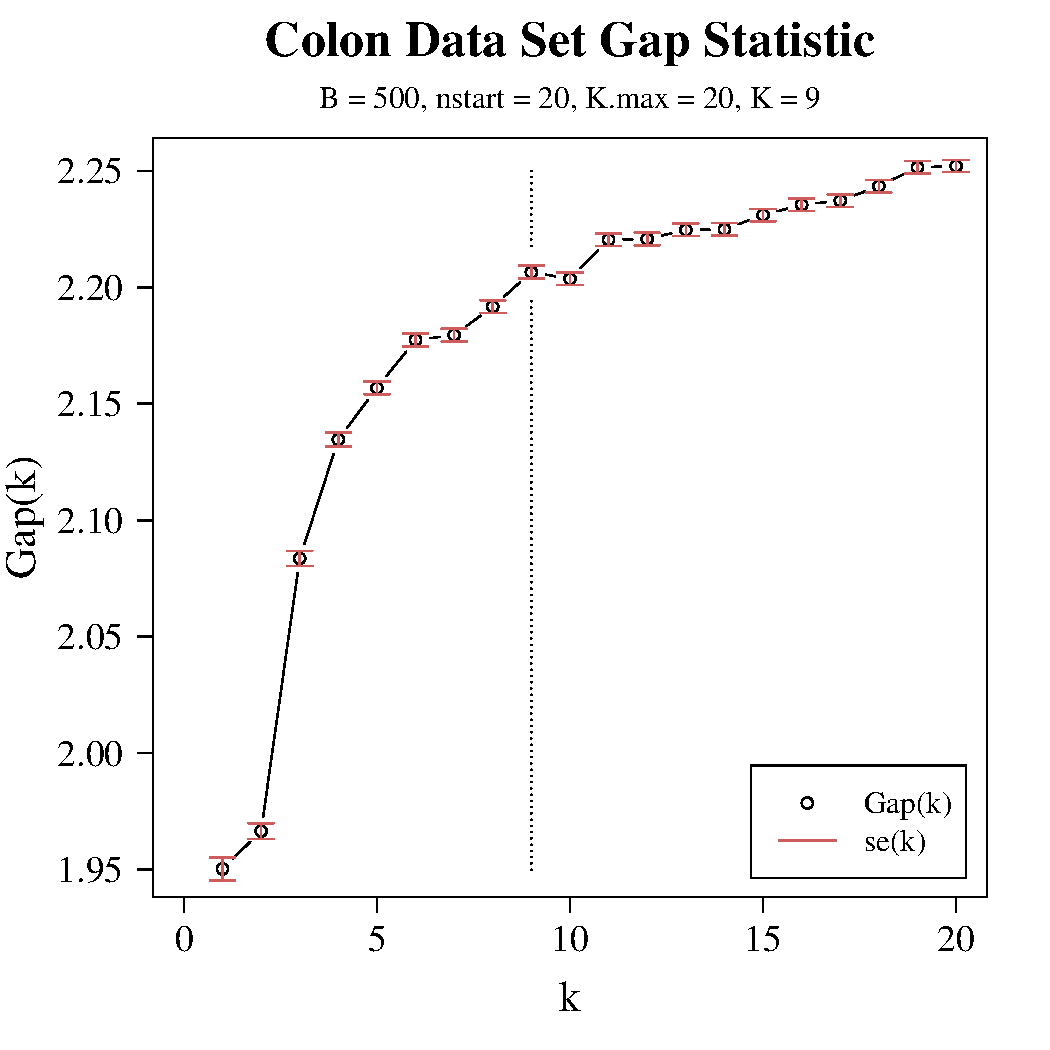
\includegraphics[width = 0.475\textwidth]{colon_gap_stat.pdf}
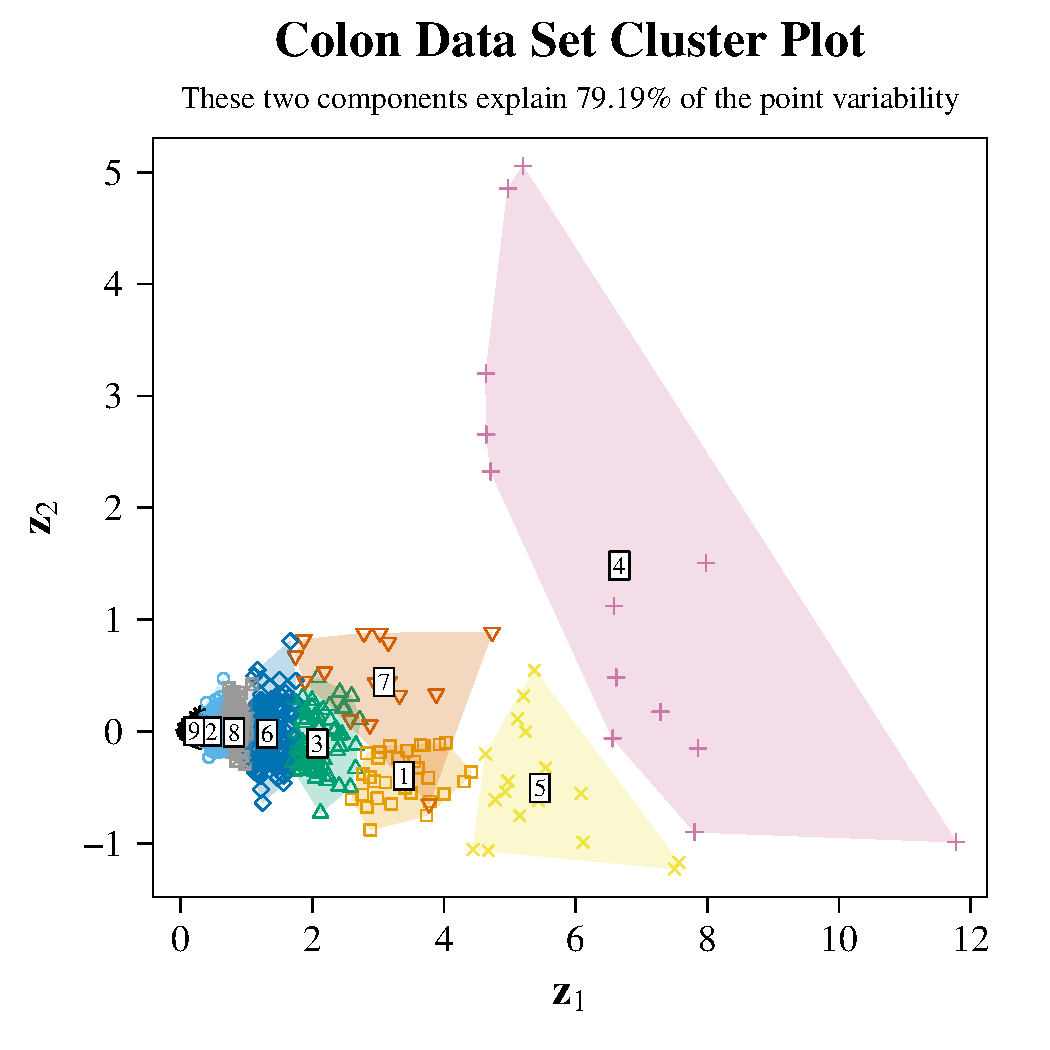
\includegraphics[width = 0.475\textwidth]{colon_clus_plot.pdf}

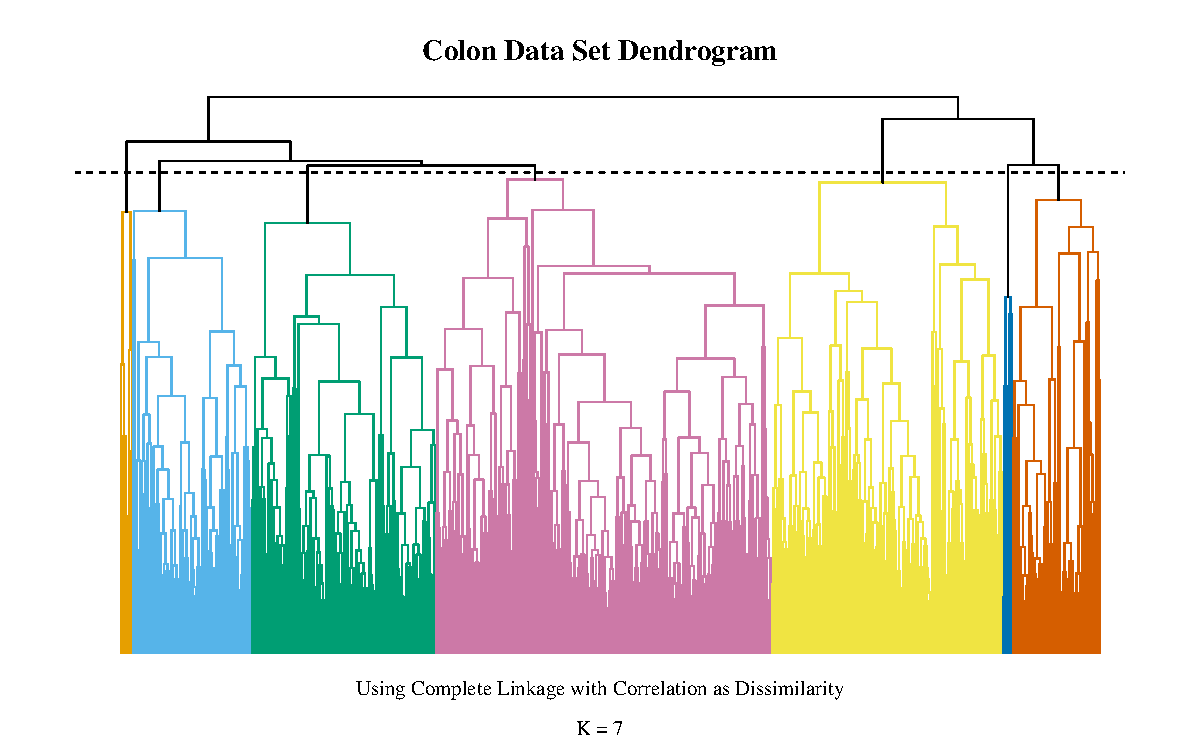
\includegraphics[width = \textwidth]{colon_den.pdf}
\caption{Clustering information for the colon data set.}
\label{colonclus}
\end{figure}

%\newpage

\begin{figure}[ht]
\centering
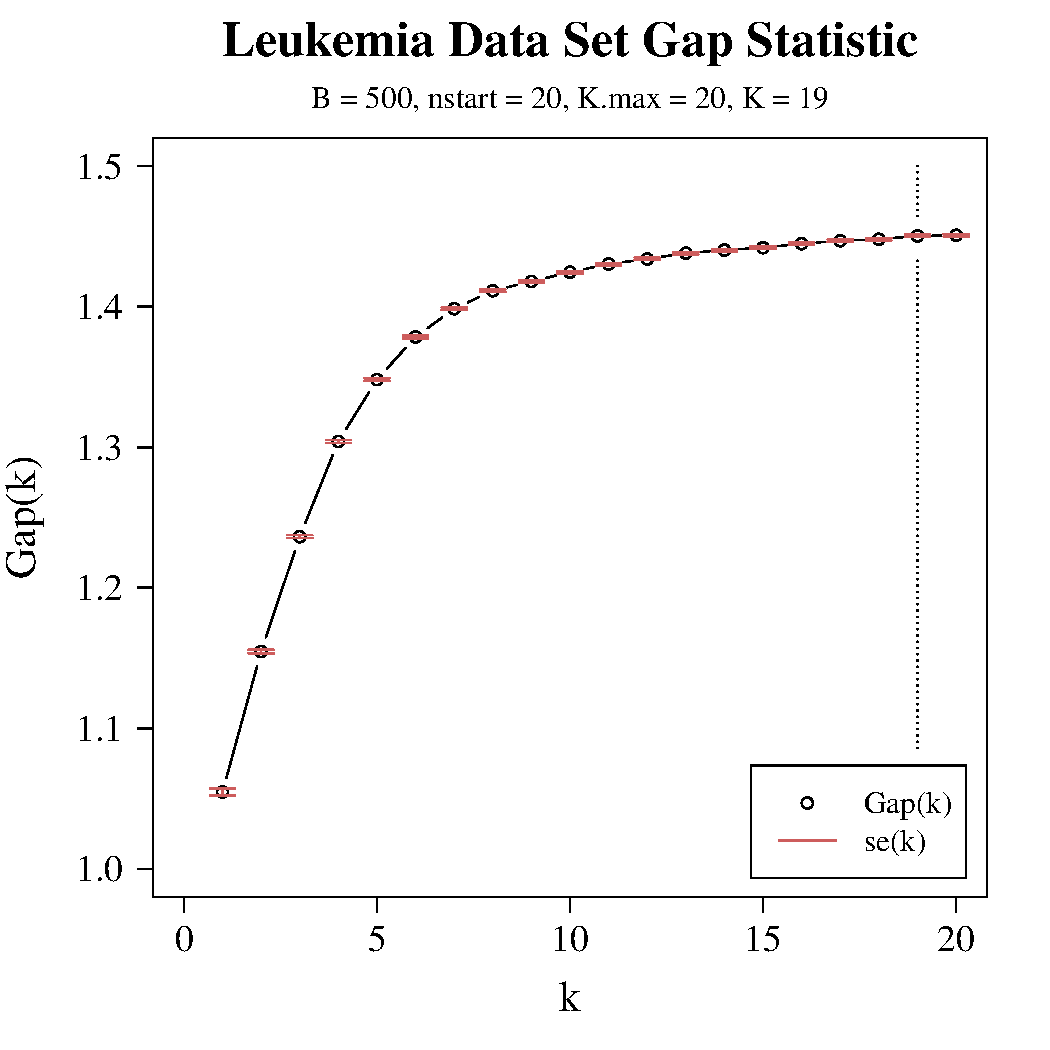
\includegraphics[width = 0.475\textwidth]{leuk_gap_stat.pdf}
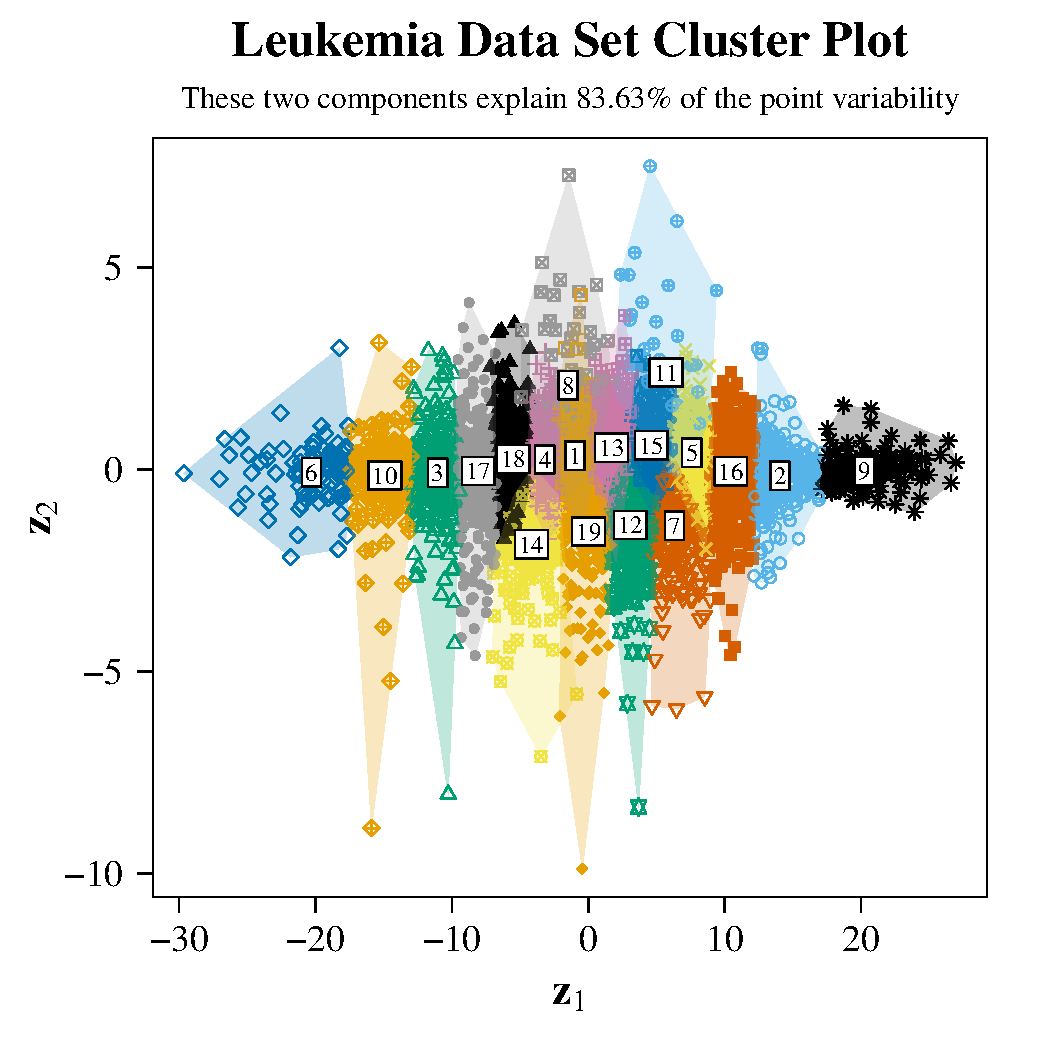
\includegraphics[width = 0.475\textwidth]{leuk_clus_plot.pdf}

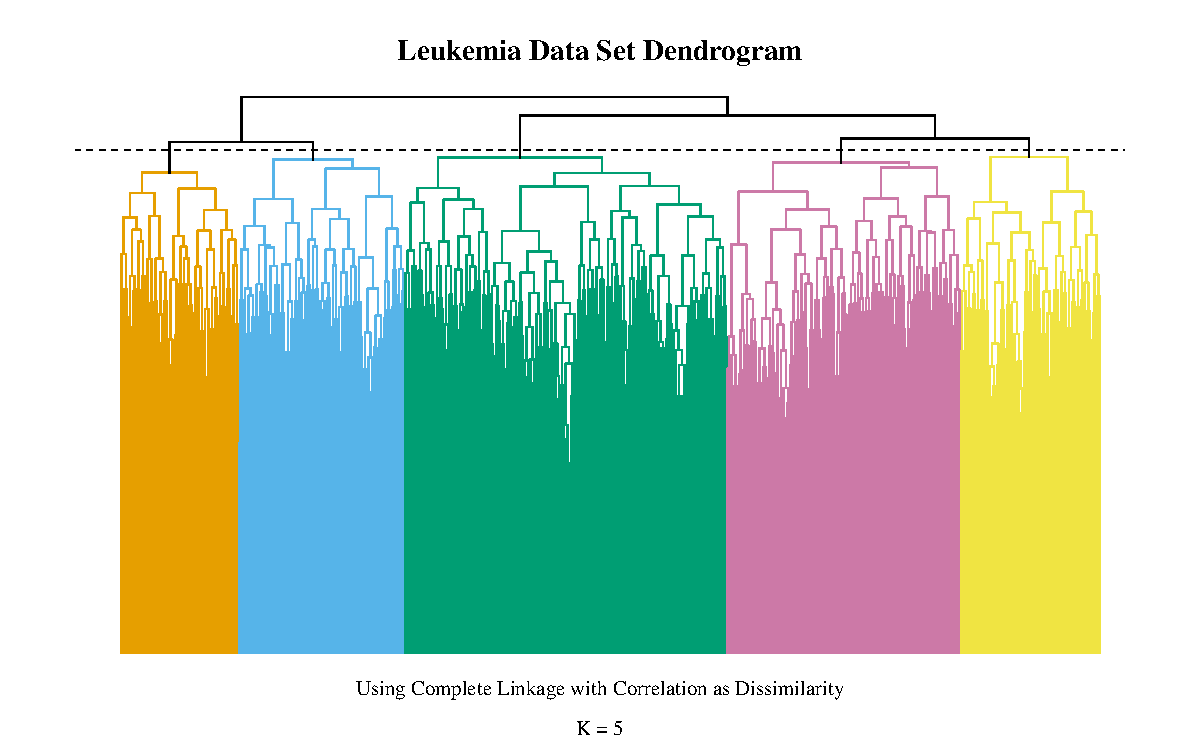
\includegraphics[width = \textwidth]{leuk_den.pdf}
\caption{Clustering information for the leukemia data set.}
\label{leukclus}
\end{figure}



\newpage
\section{Eigenvalues}

\begin{figure}[ht]
\centering
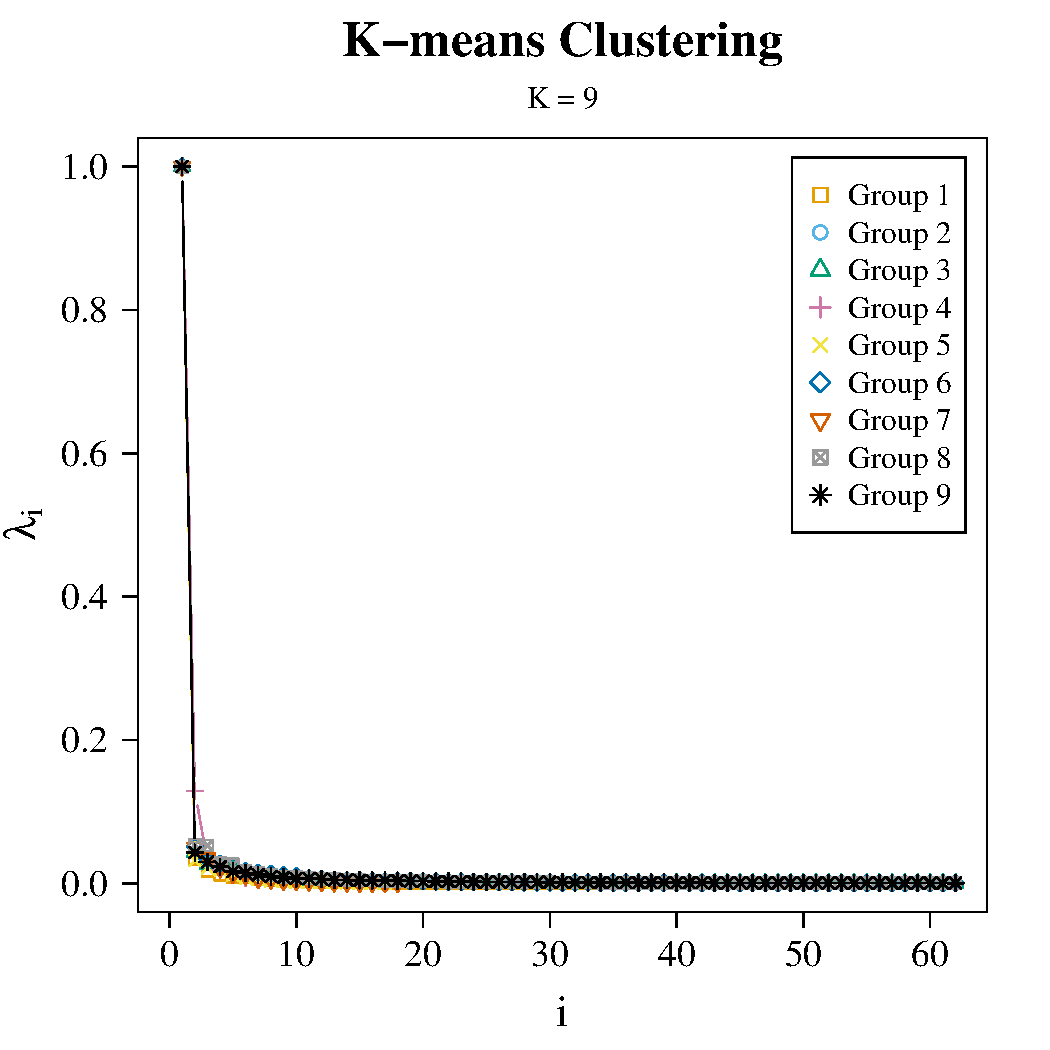
\includegraphics[width = 0.475\textwidth]{colon_eigen_k.pdf}
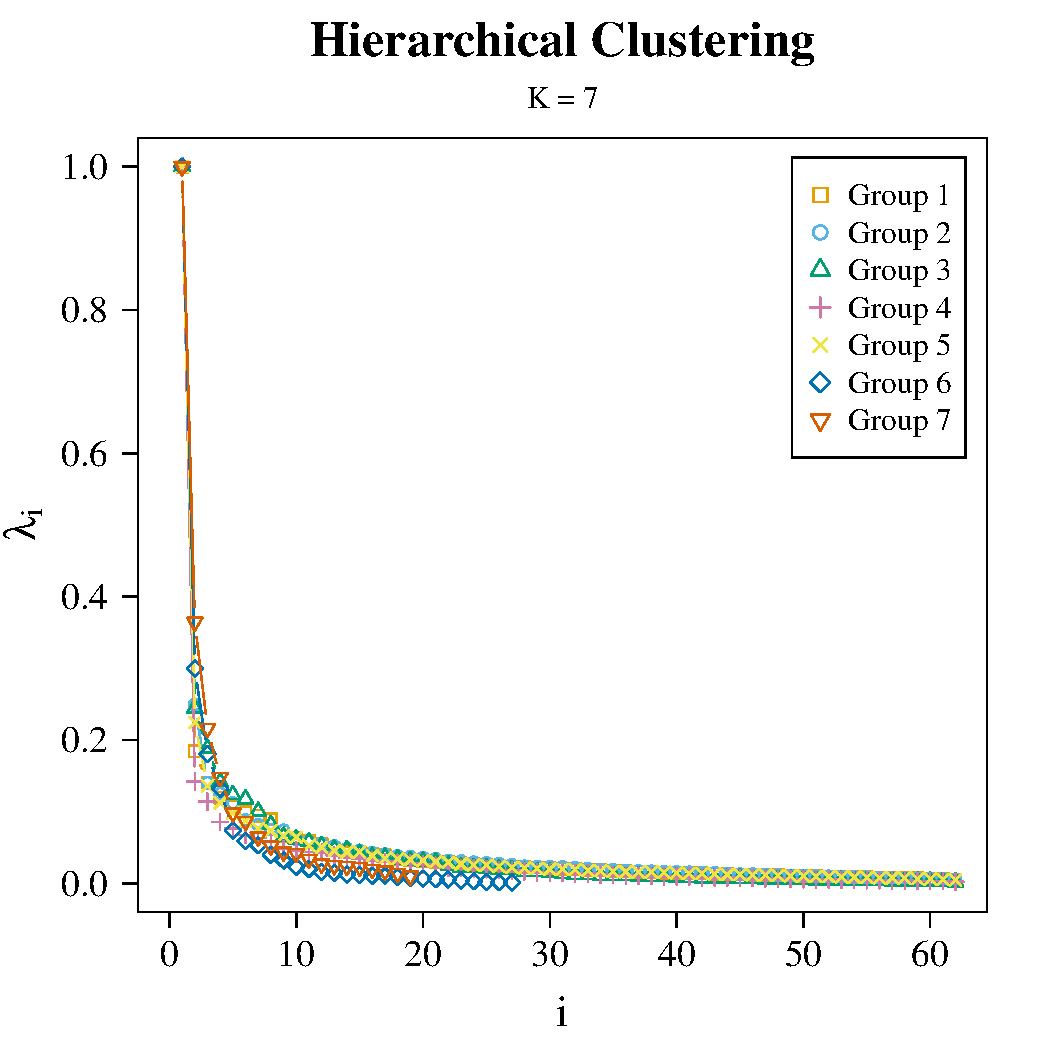
\includegraphics[width = 0.475\textwidth]{colon_eigen_h.pdf}

\caption{Covariance eigenvalues for the colon data set. The left panel uses $K$-means clustering, while the right panel uses hierarchical clustering.}
\label{coloneigen}
\end{figure}

\begin{figure}[ht]
\centering
\includegraphics[width = 0.475\textwidth]{leuk_eigen_k.pdf}
\includegraphics[width = 0.475\textwidth]{leuk_eigen_h.pdf}

\caption{Covariance eigenvalues for the leukemia data set. The left panel uses $K$-means clustering, while the right panel uses hierarchical clustering.}
\label{leukeigen}
\end{figure}


\end{document}